\section{Durchführung}
\label{sec:Durchführung}

\subsection{Aufbau}
\begin{figure}
 \centering
 \caption{Skizze der Messapparatur.}
 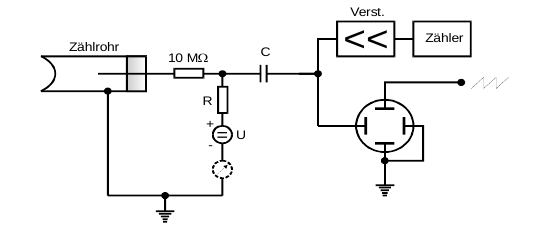
\includegraphics[width=\textwidth]{vesuchsaufbaugeiger.png}
 \label{fig:aufbauversuch}
\end{figure}

\noindent Zur Durchführung des Versuchs wurde die Versuchsanordnung verwendet,
die Abbildung \ref{fig:aufbauversuch} zeigt. Vom Anodendraht abfließende Ladung
erzeugt am Widerstand einen Spannungsimpuls, der über den Kondensator C ausgekoppelt wird,
im Verstärker vergrößert und im Zählgerät registriert, oder auf dem Schirm
eines Ozilloskops dargestellt.\\

\subsection{Charakteristik}
Um die Charakteristik des Zählrohrs aufzunehmen, wird eine Elektronenquelle vor dem
Fenster platziert. Hier wurde eine $^204Tl$-Quelle verwendet. Bei der Platzierung
wurde dabei darauf geachtet, dass bei mittlerer Spannung eine Rate von
100 Impulsen pro Sekunde nicht überschritten wurde. Dies ist erforderlich,
um Totzeit-Korrekturen zu vermeiden. \\
In 10-Volt-Schritten wurde die Anzahl an Zerfällen pro Zeitintervall gemessen, alle 
50 Volt wurde zusätzlich der Strom am Amperemeter abgelesen.\\
Die Messzeit von $t = 60\si{\s}$ wurde gewählt, um den statistischen Fehler
auf unter 1\% abzusenken, da die Empfindlichkeit dieser Messung ausgesprochen
hoch ist. 

\subsection{Totzeit}
Einmal wurde die Totzeit mithilfe des Oszilloskops bestimmt, dazu wurde 
die Zeitachse auf auf $100 \si{\micro\s}$ eingestellt.\\
Zudem wurde die Zwei-Quellen-Methode genutzt. Dazu wurde eine weitere
$^204 Tl$-Quelle verwendet, die, um eine andere Impulsrate zu erzielen,
näher am Zählrohr platziert wurde. 
